\section{Government}
	\subsection{Registration}
	There is only one government account because of its special privileges
	explained below. Developers of \textit{Soldino} are in charge of providing
	it.
	\subsection{Login}
	To log in using the government account, you have to press the \texttt{login}
	button on the top right of the homepage. The log in does not need any
	username or password since all data are retrieved via MetaMask.
	\\Log in with the correct MetaMask\glosp account is required to perform a
	successful log in.
	\subsection{Logout}
	%To log out of \textit{Soldino}, you just have to log out of 
	%MetaMask\glosp. To do this, you have to press MetaMask's icon on the top 
	%right of the browser, press your account's icon and then click on \texttt{Log out}

	To log out from \textit{Soldino}, you only have to press the \texttt{Logout}
	button on the top right of the page. To improve the security, it is
	recommended to log out also from MetaMask\glosp{}. To do so press the
	MetaMask's icon on the top right of the browser, then press your account's
	icon and finally press \texttt{Log out} on the top right.
	\begin{figure}[H]
		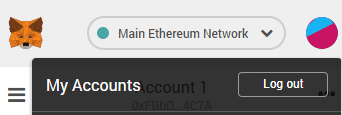
\includegraphics[width=7cm]{res/images/logout_metamask.png}
		\centering
		\caption{Logging out}
	\end{figure}
\pagebreak
	\subsection{Cubit}

	The government can mint and distribute Cubits\glosp{} by pressing the
	\texttt{Cubit Manager} button in the navigation bar, on the top of the page.
	\begin{figure}[H]
		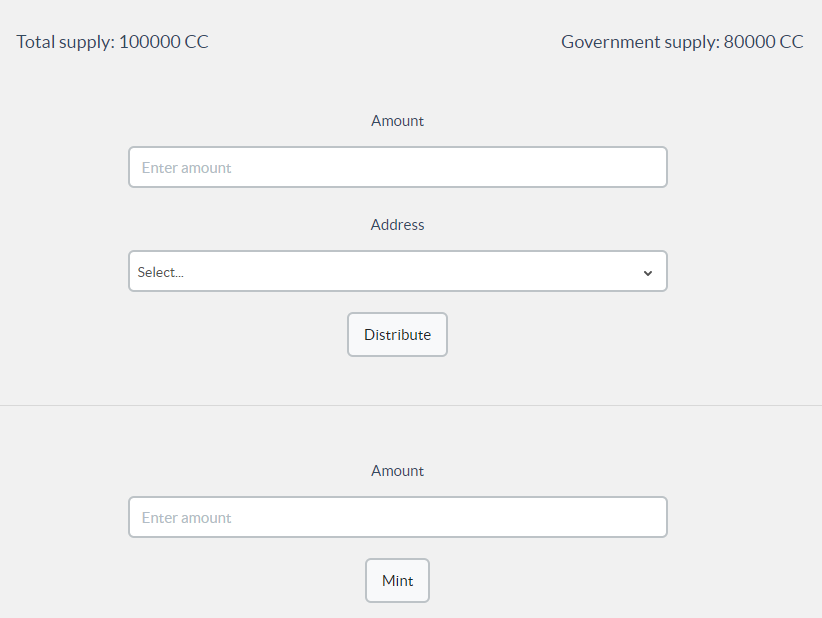
\includegraphics[width=15cm]{res/images/cubit_manager.png}
		\centering
		\caption{Government Cubit page}
	\end{figure}
		\subsubsection{Minting}
		To mint Cubits\glo{}, you have to fill the \texttt{Amount} field,
		inserting the desired quantity and then press \texttt{Mint}. After,
		you can see that the \texttt{Government supply} is increased by the
		chosen amount.
		\begin{figure}[H]
			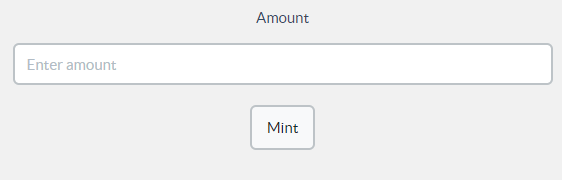
\includegraphics[width=15cm]{res/images/minting_cubits.png}
			\centering
			\caption{Minting Cubits}
		\end{figure}
		\subsubsection{Distributing}
		To distribute Cubits\glosp{} you have to insert the wanted amount in
		the \texttt{Amount} field and then select from the drop down menu the
		addresses of the accounts you wish to send the Cubits to. Every account
		you select will have a checked box next to their name. You can also
		search for an account by name using the dedicated search bar. At the
		end you have to press \texttt{Distribute}.\\
		\begin{figure}[H]
			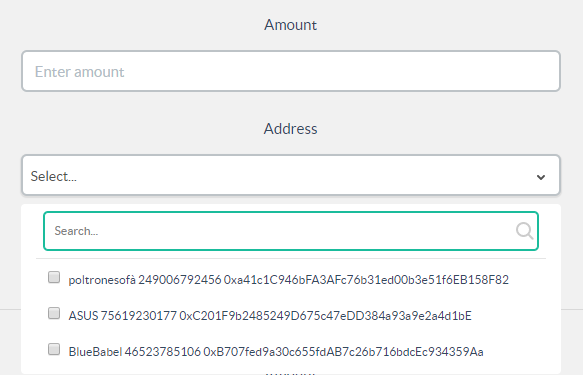
\includegraphics[width=15cm]{res/images/distributing.png}
			\centering
			\caption{Distributing Cubits}
		\end{figure} \mbox{}\\
		\noindent Note that the amount of cubits distributed must be lower than
		the \texttt{Government supply} otherwise you will not be able to send
		them.
	\subsection{Managing users}
	The government can reactivate disabled accounts or deactivate active 
	accounts. This can be done by clicking on the \texttt{Citizens List} or 
	\texttt{Businesses List} in the navigation bar on the top of the page 
	where all \textit{Soldino} users' information can be found.
	\begin{figure}[H]
		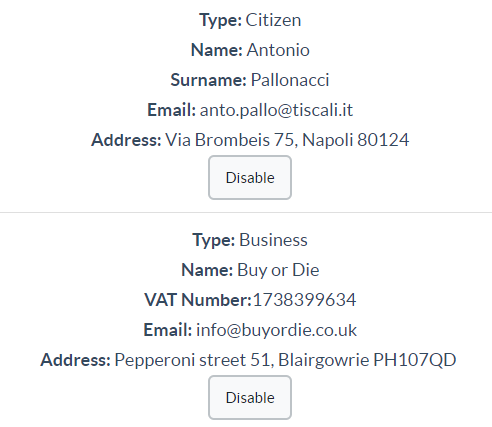
\includegraphics[width=13cm]{res/images/users_list.png}
		\centering
		\caption{Example of users list}
	\end{figure}
		\subsubsection{Deactivating users}
		Once you have found the account that you want to disable, press the 
		\texttt{Disable} button. Disabling an account means that it will no 
		longer be able log into \textit{Soldino} until it will be enabled again.
		\begin{figure}[H]
			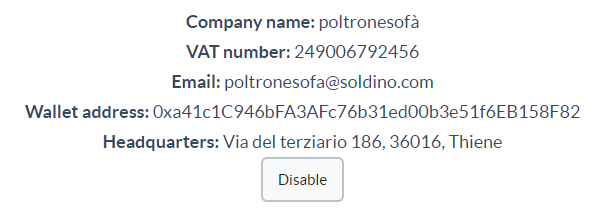
\includegraphics[width=15cm]{res/images/user_disable.png}
			\centering
			\caption{Example of disabling an activated account}
		\end{figure}
		\subsubsection{Activating users}
		Once you have found the account that you want to enable, press the
		button \texttt{Enable}. After being enabled, an account can log onto 
		\textit{Soldino} again.
		\begin{figure}[H]
			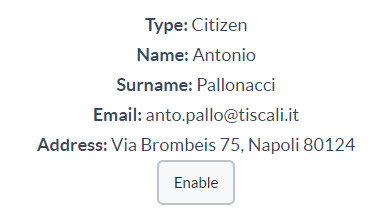
\includegraphics[width=15cm]{res/images/user_enable.png}
			\centering
			\caption{Example of enabling a deactivated account}
		\end{figure}
	\subsection{Refund VAT}
	You can see all businesses registered on the platform and their Vat status
	by press the \texttt{VAT Refund} button in the navigation bar on the top of 
	the page. 
	\begin{figure}[H]
		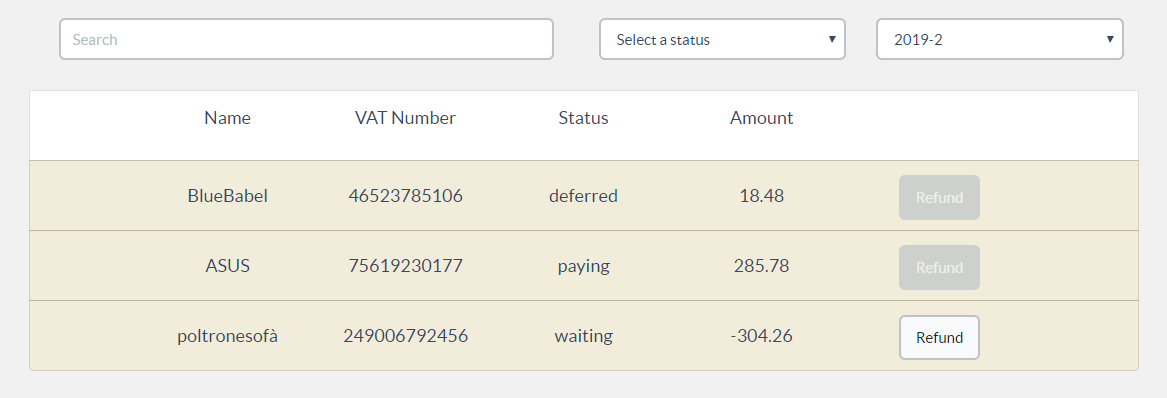
\includegraphics[width=15cm]{res/images/business_list.png}
		\centering
		\caption{List of Business}
	\end{figure}
	\noindent From this page you will be able to search for businesses by their
	name or to filter them by their VAT status using the 
	\texttt{Select a status} drop down menu.
	\begin{figure}[H]
		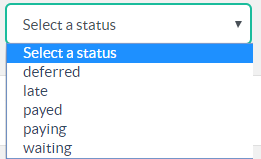
\includegraphics[width=7cm]{res/images/vat_status_select.png}
		\centering
		\caption{Select a status to filter the businesses}
	\end{figure}
	\noindent Press \texttt{Refund} to refund a business that has
	\texttt{Waiting} status.\\
	You can check previous quarters by using the \texttt{Select a period}
	drop down menu on the right.
%	\begin{figure}[H]
%		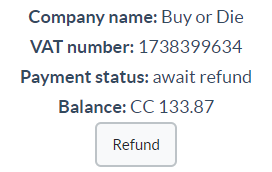
\includegraphics[width=7cm]{res/images/business_refund.png}
%		\centering
%		\caption{Example of reimbursing a business}
%	\end{figure}